\documentclass[10pt,twocolumn,letterpaper]{article}

\usepackage{cvpr}
\usepackage{times}
\usepackage{epsfig}
\usepackage{graphicx}
\usepackage{amsmath}
\usepackage{amssymb}
\usepackage{booktabs}
\usepackage{microtype}
\usepackage{multirow}
\usepackage{xcolor}
\usepackage[pagebackref,breaklinks,colorlinks]{hyperref}

\definecolor{cvprblue}{rgb}{0.21,0.49,0.74}
\hypersetup{colorlinks=true,breaklinks=true,linkcolor=cvprblue,citecolor=cvprblue,urlcolor=cvprblue}

\newcommand{\method}[1]{\textsc{#1}}
\newcommand{\biou}{\mathrm{BIoU}}
\newcommand{\miou}{\mathrm{mIoU}}

\title{Boundary-Aware Agricultural Field Segmentation:\\
Where Should Boundary Supervision Enter?}

\author{Arian Norouzi \qquad Xiyang Lyu \qquad Yelyzaveta Tryfonova\\
Team 004, High-Level Computer Vision\\
Saarland University\\
{\tt\small 7061871 \qquad 7058370 \qquad 7072789}}

\begin{document}
\maketitle

\begin{abstract}
Binary agricultural-field segmentation can recover the correct cultivated area while merging neighboring parcels across narrow gaps. We study where boundary information should enter a compact U-Net trained on multi-date Sentinel-2 imagery: directly in the mask loss, indirectly through signed-distance-field (SDF) regression, or through an explicit boundary-classification head. All variants share the same backbone, Fields of The World subset, augmentation, and held-out test set. At a common probability threshold of 0.60, a mask-only BCE+Dice baseline obtains 0.6572 mean IoU and 0.3469 Boundary IoU. Boundary-weighted BCE raises these scores to 0.6675 and 0.3926. A boundary-focused SDF auxiliary task provides only a small Boundary-IoU gain (0.3501) and reduces mean IoU to 0.6499. Combining boundary-weighted mask training with an explicit boundary head gives the best Boundary IoU, 0.4000, while retaining 0.6634 mean IoU. These results favor direct supervision of the final mask and boundary features over indirect distance regression for this setting, although the single-seed, three-country evaluation limits the strength of the conclusion.
\end{abstract}

\section{Introduction}
Agricultural field boundaries are useful units for crop monitoring, yield estimation, policy, and resource planning, yet manual delineation is expensive. The Fields of The World (FTW) benchmark addresses this problem with multi-date Sentinel-2 imagery and both semantic and instance labels across 24 countries~\cite{kerner2025ftw}. Its binary target is suitable for foreground segmentation, but it obscures a structural failure mode: two adjacent fields can be predicted as one connected region while most foreground pixels remain correct. Region IoU may therefore understate practically important errors along thin parcel borders.

Figure~\ref{fig:problem} illustrates the gap between semantic area and parcel structure. The instance labels identify many separate fields whose borders occupy only a small fraction of the image. Standard pixel losses are dominated by interiors and background, so a model may have little incentive to preserve these narrow separations. We ask a focused question: \emph{where should boundary information enter learning if the final output remains a binary field mask?}

We compare three interventions against the same mask-only U-Net. First, boundary-weighted BCE directly increases the gradient contribution of mask pixels near instance boundaries. Second, SDF regression introduces an auxiliary geometry task whose error is concentrated near the zero level set. Third, a boundary head explicitly classifies a narrow border band while sharing features with the mask decoder. Our contribution is the controlled comparison rather than a new backbone. On 1,430 held-out chips from Austria, Croatia, and Denmark, direct mask weighting produces most of the gain, and the explicit boundary head provides a further improvement in Boundary IoU. The SDF auxiliary task is less effective and slightly harms region overlap.

\begin{figure}[t]
  \centering
  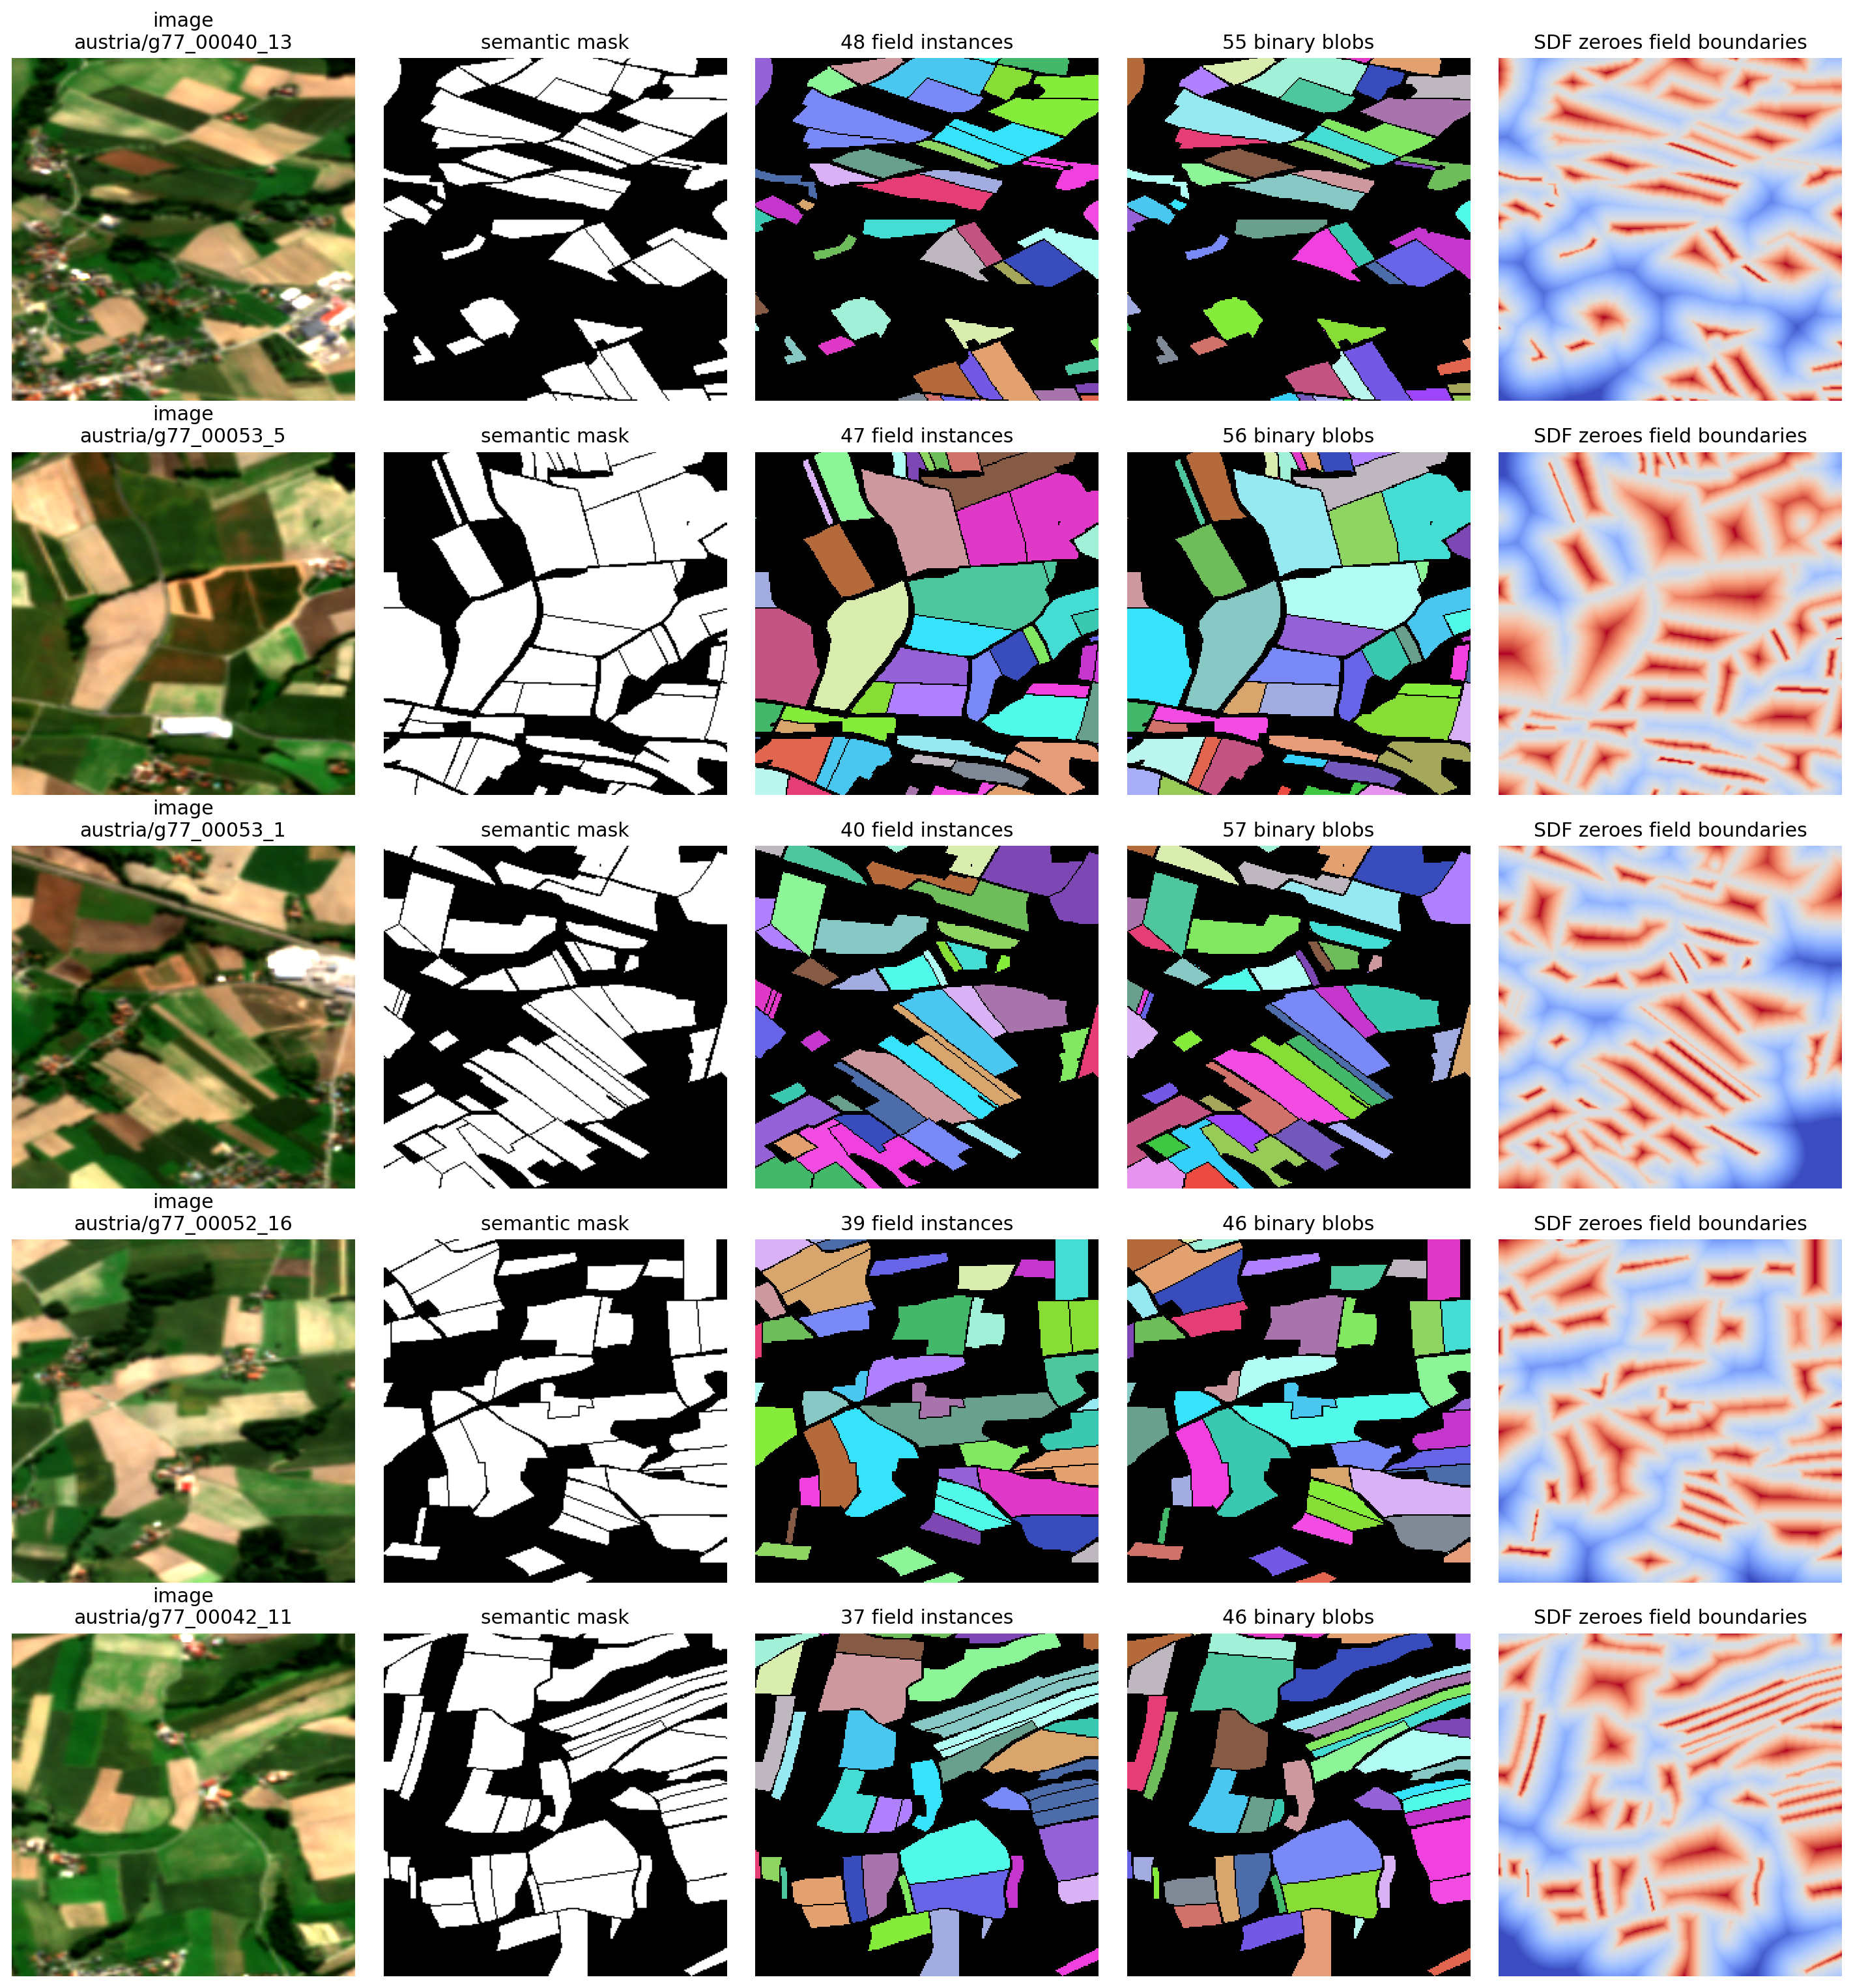
\includegraphics[width=\linewidth]{../Visualizations/problem_setup/val_blob_issue.png}
  \caption{A semantic field mask (center) contains little information about which foreground pixels belong to distinct parcels (right). Instance labels are used only to derive boundary-aware training targets.}
  \label{fig:problem}
\end{figure}

\section{Related Work}
\textbf{Field segmentation.} FTW contains 70,462 samples with multi-date, multispectral Sentinel-2 imagery and semantic and instance masks~\cite{kerner2025ftw}. We use only its Austria--Croatia--Denmark subset and evaluate in-domain rather than testing geographic generalization.

\textbf{Dense prediction and auxiliary heads.} U-Net uses skip-connected decoding for precise localization~\cite{ronneberger2015unet}. A shared backbone with separate heads is hard-parameter-sharing multi-task learning: related targets can act as an inductive bias that improves generalization~\cite{caruana1997multitask}, although performance depends on loss balance~\cite{kendall2018multitask}. For boundary-aware segmentation, Bischke et al. jointly predict building masks and boundaries in overhead imagery~\cite{bischke2019buildings}, while Zhen et al. couple semantic masks with boundary detection~\cite{zhen2020joint}. These results motivate our lightweight two-head variant, but do not guarantee transfer. Our SDF branch instead follows distance-transform boundary losses that address the imbalance between region and contour pixels~\cite{kervadec2021boundary}.

\textbf{Evaluation.} Boundary IoU was introduced because ordinary mask IoU can be insensitive to contour quality~\cite{cheng2021boundaryiou}. We adapt it to semantic masks by computing IoU between symmetric bands around the predicted and target contours, and report it beside per-image mean region IoU.

\section{Method}
\subsection{Data representation and shared backbone}
Each $256\!\times\!256$ chip contains red, green, blue, and near-infrared bands from two seasonal windows, concatenated into an eight-channel input. Reflectance values are scaled and clipped to $[0,1]$. The backbone is a U-Net with base width 32, four downsampling and four upsampling stages, transposed-convolution upsampling, and skip connections. The mask-only model has 7.76M trainable parameters; either auxiliary head adds about 9.3K parameters (0.12\%). No pretrained encoder is used.

Let $Y_i\in\{0,1\}$ be the semantic target and $z_i$ the mask logit. From the FTW instance mask we compute an SDF $D_i\in[-1,1]$. Distances are positive inside each field and normalized per instance, zero at its boundary, and negative in the background with outside distances clipped at 32 pixels. Thus touching field instances retain separate zero level sets even when their semantic class is identical.

All methods include Dice loss~\cite{milletari2016vnet},
\begin{equation}
  \mathcal{L}_{\mathrm{Dice}}=1-\frac{2\sum_i p_iY_i+\epsilon}{\sum_i p_i+\sum_iY_i+\epsilon},
  \qquad p_i=\sigma(z_i),
\end{equation}
with BCE for local classification. Total-variation code is available in the implementation but its weight is zero in the reported configurations.

\subsection{Direct boundary weighting}
The first intervention modifies BCE on the final mask output. Pixels near the SDF zero level set receive
\begin{equation}
  w_i=1+\alpha\exp\left(-|D_i|/\tau\right),
  \quad \alpha=20,\quad \tau=0.12,
\end{equation}
and the normalized loss is
\begin{equation}
  \mathcal{L}_{\mathrm{WBCE}}=
  \frac{\sum_i w_i\,\mathrm{BCE}(z_i,Y_i)}{\sum_i w_i}.
\end{equation}
The weight equals 21 on a boundary, 8.36 at $|D|=0.12$, and approaches one far away. The objective is $\mathcal{L}_{\mathrm{WBCE}}+\mathcal{L}_{\mathrm{Dice}}$. Because the weighting acts on mask logits, boundary mistakes directly influence the prediction used at inference.

\subsection{Boundary-focused SDF regression}
The second intervention adds a distance head $z^D$ to the shared decoder. Its $\tanh$ output matches the normalized SDF range, and Smooth L1 limits the influence of large distance errors. The experiment uses
\begin{align}
  a_i &= \exp\left(-|D_i|/\tau\right),\\
  \mathcal{L}_{\mathrm{WSDF}} &=
  \frac{\sum_i a_i\,\mathrm{SmoothL1}(\tanh z_i^D,D_i)}{\sum_i a_i},\\
  \mathcal{L}_{\mathrm{SDF}} &= \mathcal{L}_{\mathrm{BCE}}+
  \mathcal{L}_{\mathrm{Dice}}+0.5\mathcal{L}_{\mathrm{WSDF}}.
\end{align}
The hypothesis is multi-task learning: accurate local geometry should improve the features shared with the mask head. Only the mask output is used for the reported segmentation.

\subsection{Explicit boundary prediction}
The final model combines direct mask weighting with a second active head that predicts
\begin{equation}
  B_i=\mathbf{1}\left[|D_i|\leq0.12\right].
\end{equation}
Because the positive boundary band is thin, the boundary BCE uses a batch-wise positive-class weight equal to the negative-to-positive pixel ratio, clipped at 50. Its objective is
\begin{equation}
  \mathcal{L}_{M+B}=\mathcal{L}_{\mathrm{WBCE}}+
  \mathcal{L}_{\mathrm{Dice}}+2\mathcal{L}^{\mathrm{bal}}_{\mathrm{BCE}}(z^B,B).
\end{equation}
This head explicitly teaches shared features which pixels form borders, but the final binary segmentation still comes from the mask head. The heads interact only through the shared decoder and summed training loss, and mask inference is unchanged.

\section{Experimental Setup}
\textbf{Data.} We use the official FTW splits for Austria, Croatia, and Denmark: 10,938 training, 1,347 validation, and 1,430 test chips. Training applies horizontal and vertical flips, rotations, mild affine translation and scaling, RGB brightness/contrast jitter, Gaussian blur and noise, and random erasing. Validation and test inputs are not augmented.

\textbf{Optimization and selection.} Models are trained from scratch on one GPU with batch size 16 using AdamW~\cite{loshchilov2019adamw}, learning rate $2\!\times\!10^{-4}$, weight decay $10^{-3}$, and cosine annealing. Runs last up to 60 epochs. The validation Boundary IoU selects one checkpoint per configuration; the test set is then used for the final comparison. This protocol separates model selection from final reporting.

\textbf{Metrics.} At inference, mask probabilities are thresholded at a common 0.60. We report per-image mean foreground IoU. For Boundary IoU, each binary mask $M$ is converted to a symmetric band
\begin{equation}
  \partial_r M=\mathrm{dilate}(M,r)-\mathrm{erode}(M,r),\qquad r=1.
\end{equation}
The band extends one pixel inward and outward (approximately 20 m total width at 10 m resolution). We then compute IoU between predicted and target bands and average over images. A common threshold avoids tuning a separate test operating point for each model.

\section{Results and Analysis}
\begin{table}[t]
\centering
\caption{Held-out test results on 1,430 chips at threshold 0.60. Best is bold; second best is underlined. ``Gain'' is the absolute Boundary-IoU change from the baseline.}
\label{tab:results}
\small
\setlength{\tabcolsep}{3.2pt}
\begin{tabular}{@{}lrrr@{}}
\toprule
Method & $\miou$ & $\biou$ & $\Delta\biou$ \\
\midrule
Mask baseline & 0.6572 & 0.3469 & -- \\
Boundary-weighted BCE & \textbf{0.6675} & \underline{0.3926} & +0.0457 \\
Weighted SDF head ($\lambda=.5$) & 0.6499 & 0.3501 & +0.0032 \\
Mask + boundary head & \underline{0.6634} & \textbf{0.4000} & +0.0531 \\
\bottomrule
\end{tabular}
\end{table}

Table~\ref{tab:results} shows a clear difference between indirect and direct boundary supervision. Boundary-weighted BCE improves Boundary IoU by 4.57 percentage points and mIoU by 1.03 points over the mask baseline. Thus emphasizing difficult mask pixels near borders does not merely trade interior accuracy for contours; in this run it improves both.

The boundary-focused SDF head gives only a 0.32-point Boundary-IoU gain while reducing mIoU by 0.73 points. The auxiliary regression objective may spend capacity modeling distance magnitudes that are not required for a binary decision. Moreover, per-instance normalization makes equal SDF values correspond to different physical distances for differently sized fields. These are plausible explanations, not isolated causal conclusions.

Adding explicit boundary classification on top of weighted mask training reaches the best Boundary IoU, 0.4000. Its 0.74-point gain over boundary-weighted BCE suggests that a dedicated border task provides information beyond reweighting mask gradients. Its mIoU, 0.6634, remains 0.62 points above baseline but is 0.41 points below boundary-weighted BCE. The preferred model therefore depends on whether boundary fidelity or region overlap is prioritized. Across thresholds 0.40, 0.50, 0.60, and 0.70, the explicit-head model also retains the best Boundary IoU, reducing the chance that the conclusion is an artifact of the chosen operating point.

\begin{figure}[t]
\centering
\setlength{\tabcolsep}{1pt}
\begin{tabular}{ccc}
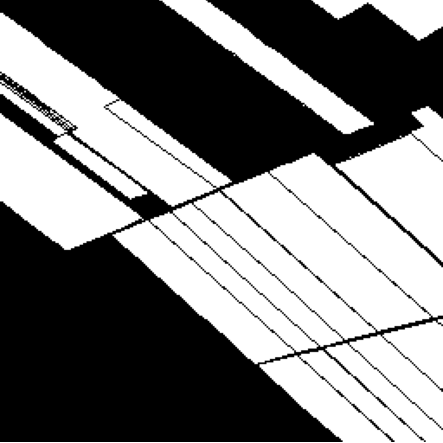
\includegraphics[width=.31\linewidth]{../Visualizations/sample_austria_g83_00040_14/ground_truth_mask.png} &
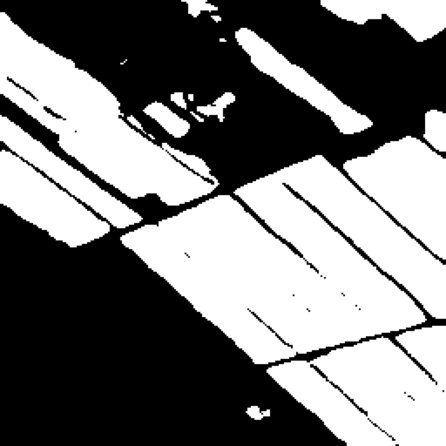
\includegraphics[width=.31\linewidth]{../Visualizations/presentation_comparison/baseline_mask.png} &

\includegraphics[width=.31\linewidth]{../Visualizations/presentation_comparison/mask_boundary_heads_mask.png} \\
\scriptsize Ground truth & \scriptsize Baseline & \scriptsize BCE + boundary
\end{tabular}
\caption{Qualitative comparison on the same Austria validation chip at threshold 0.60. The best boundary model preserves more thin separations than the baseline, but local artifacts remain. Quantitative claims use the complete held-out test set.}
\label{fig:qualitative}
\end{figure}

Figure~\ref{fig:qualitative} qualitatively matches the aggregate result: the baseline merges or erodes several narrow separations, while direct supervision recovers more internal field edges. The example also cautions against overclaiming. None of the binary outputs reconstructs the instance map, and improved contour overlap does not guarantee topologically correct parcels.

\subsection{Limitations}
Each configuration is a single run, so small differences may reflect optimization noise. The three-country subset does not test cross-country generalization; the cited multi-task literature motivates rather than establishes such transfer. Loss weights and band width were not exhaustively tuned. Boundary IoU omits instance count, connectivity, and polygon validity, while the threshold study changes only the operating point. Future work should repeat seeds, report per-country results, add instance-level metrics, and test boundary-guided post-processing.

\section{Conclusion}
For binary agricultural field segmentation in this controlled FTW experiment, boundary information is most useful when it acts directly on the mask objective and on an explicit border task. Boundary-weighted BCE supplies most of the improvement and achieves the highest mIoU, while the added boundary head yields the best Boundary IoU. Boundary-focused SDF regression provides much less benefit and slightly reduces region overlap. The evidence supports direct boundary supervision for this setting, while the limited geographic scope and single-seed runs leave broader generalization to future work.

\section*{Appendix: Team Contributions}
\textbf{Arian Norouzi:} pipeline, SDF objectives, evaluation/visuals, presentation, and report. \textbf{Xiyang Lyu:} configurations, training/checkpoints, comparisons, and boundary-head experiments. \textbf{Yelyzaveta Tryfonova:} loader, SDF caching/runtime, and debugging.

\clearpage
{\small
\bibliographystyle{ieee_fullname}
\bibliography{references}
}

\end{document}
